Die Abbildung \ref{fig:diagrammInitial_worp} zeigt grafisch die Ergebnisse der
Messreihen für den initialen Durchlauf ohne relevante Bereiche. Dabei ist die
Laufzeit in $µs$ über die Textgröße in Byte logarithmisch aufgetragen. Für
relativ kleine Textgrößen hat die Geschwindigkeitsoptimierung noch keine großen
Einfluss. Erst bei einer Größe von $5.000.000$ ($99$ µs) oder
$10.000.000$ ($122$ µs) Byte ist der erwartete Geschwindigkeitsprofit zu
verzeichnen.

\begin{figure}[H]
	\centering
	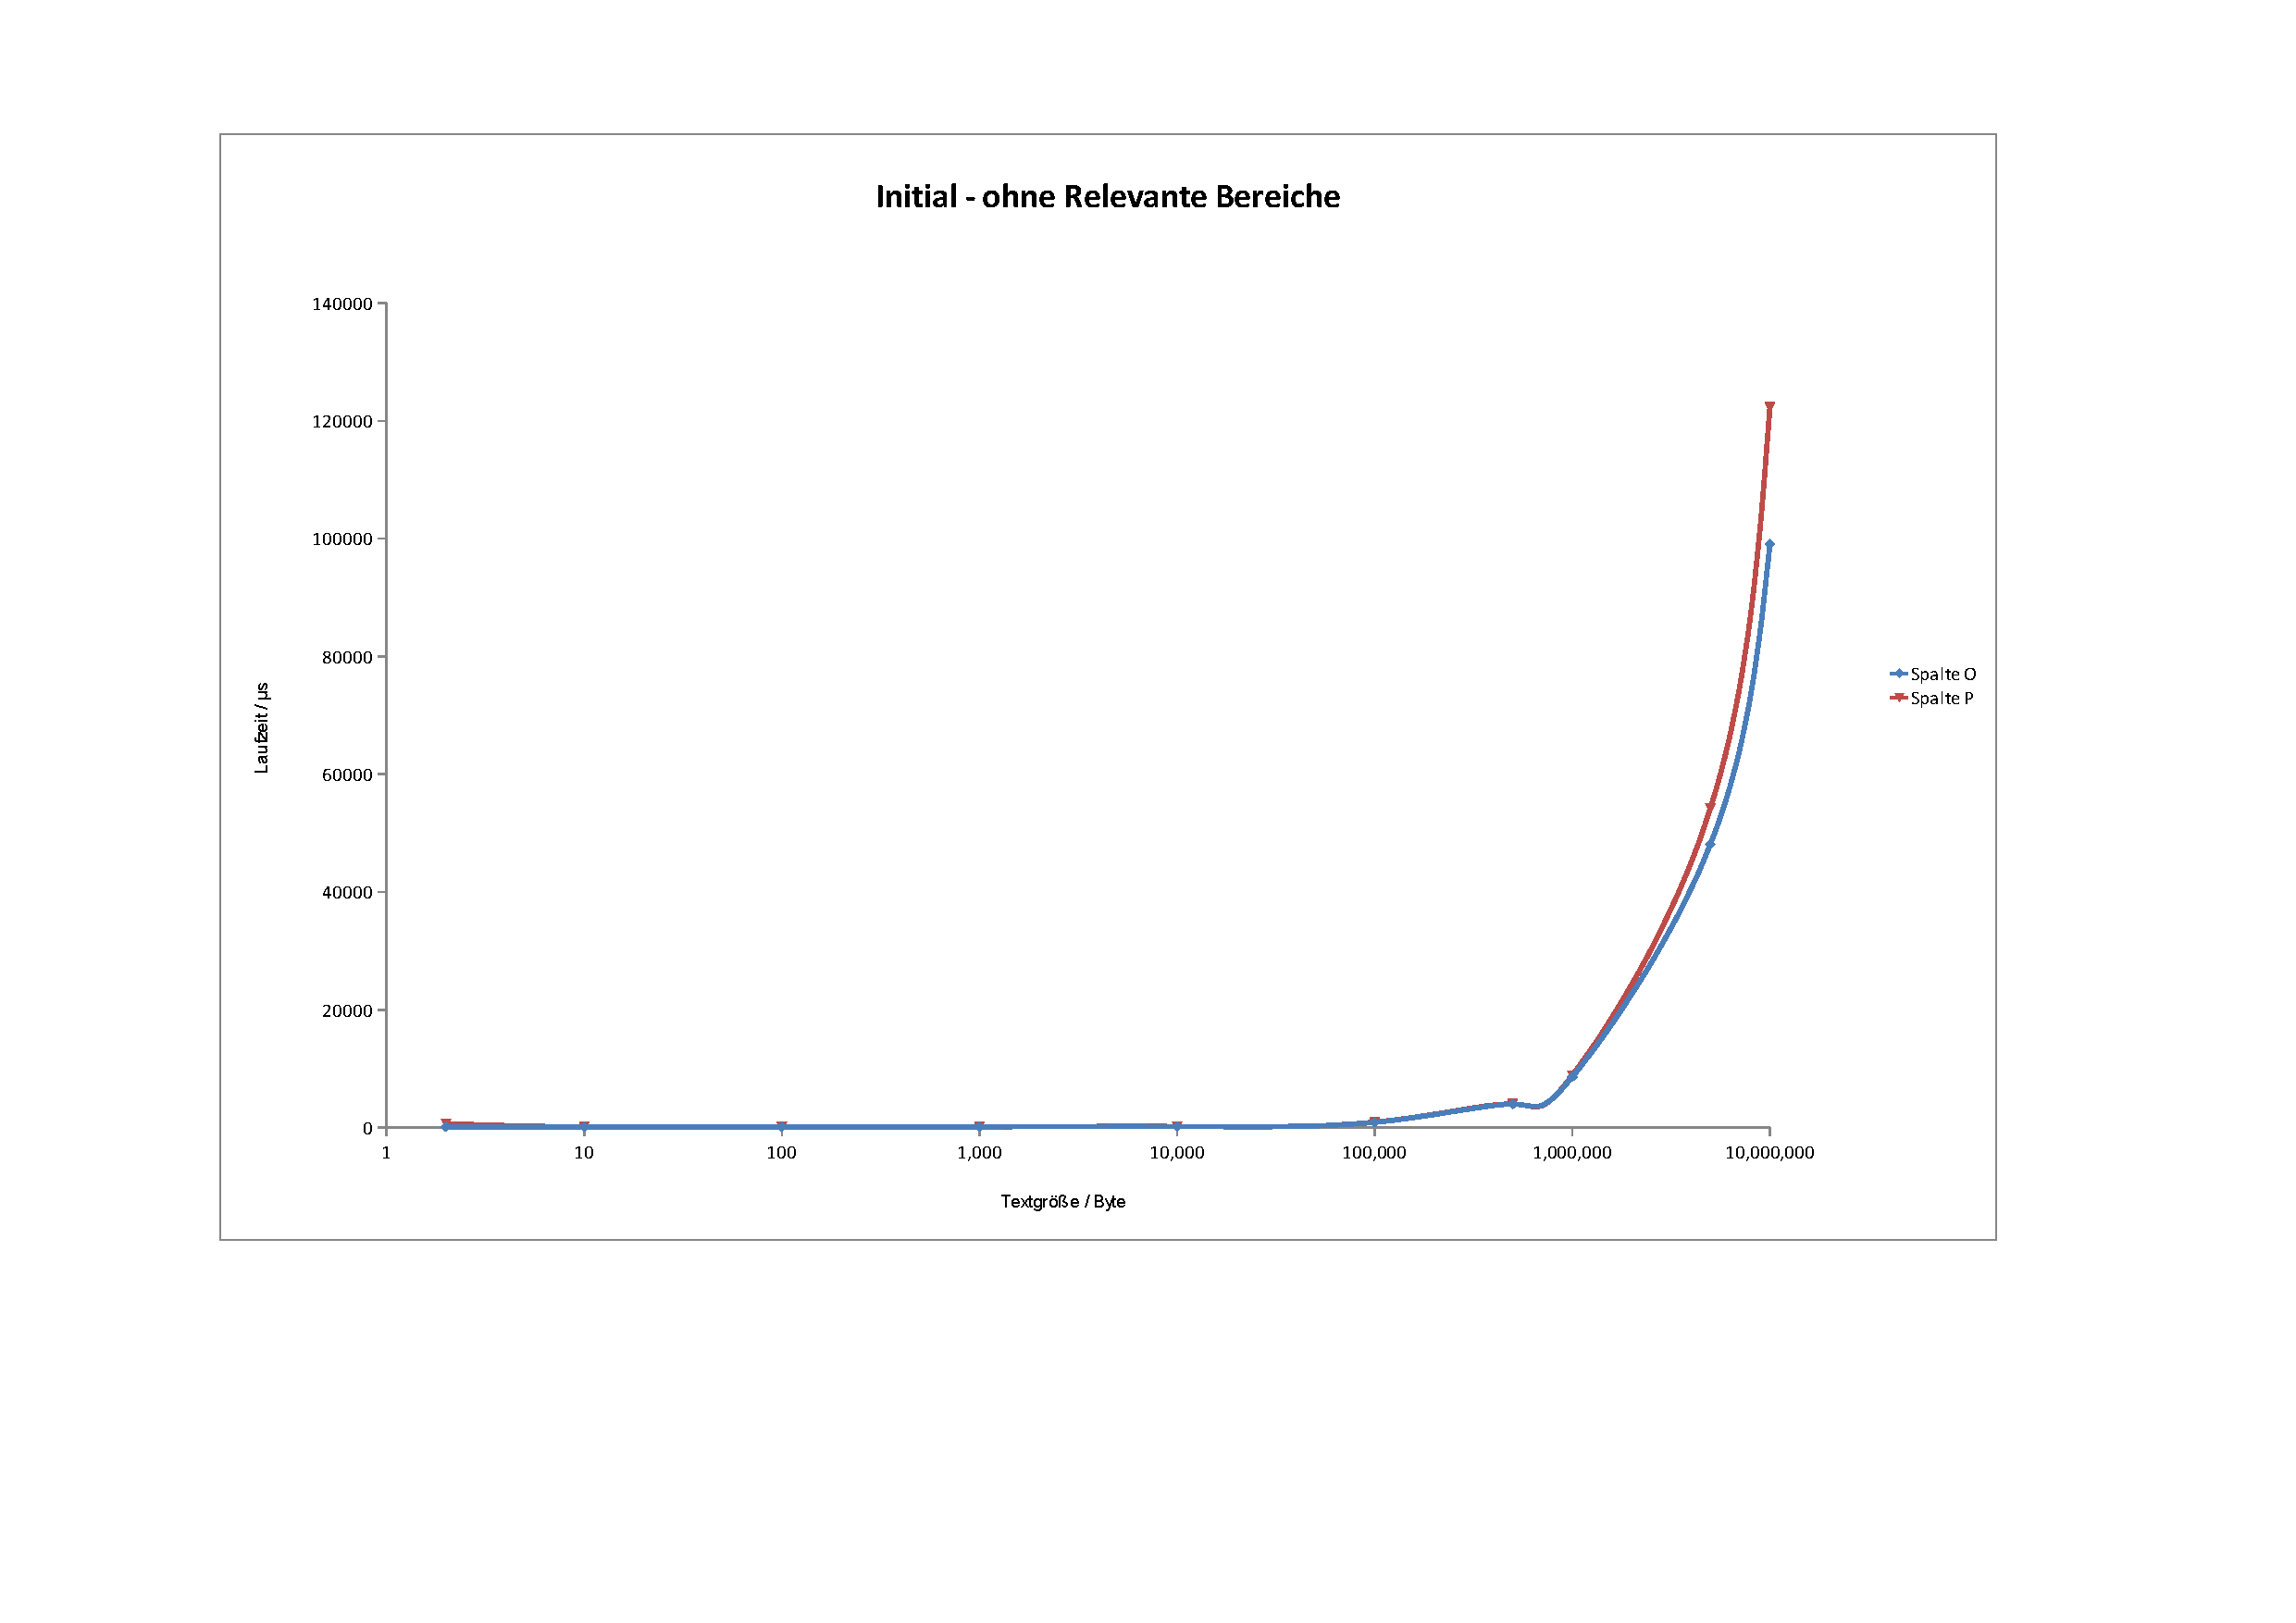
\includegraphics[scale=.45]{DiagrammInitial_worp.pdf}
	\label{fig:diagrammInitial_worp}
	\caption{Messung-Initial ohne relevante Bereiche}
\end{figure}

Der Nachteil gegenüber der Quellcodegrößenoptimierung liegt darin, dass
mehr Speicherplatz in Anspruch genommen wird, wodurch der
Geschwindigkeitsvorteil erreicht werden kann.
Die Wahl der jeweiligen Optmierungsmöglichkeit ist situationsabhängig. Auf dem
Mars stehen weniger Speicherressourcen zur Verfügung, wodurch eine
Geschwindigkeitsoptimierung weniger sinnvoll erscheint. Die gleichen
Betrachtungen ergeben sich für alle anderen Messreihen (Abbildung im Anhang
\ref{sec:Diagramme}). 

\begin{figure}[H]
	\centering
	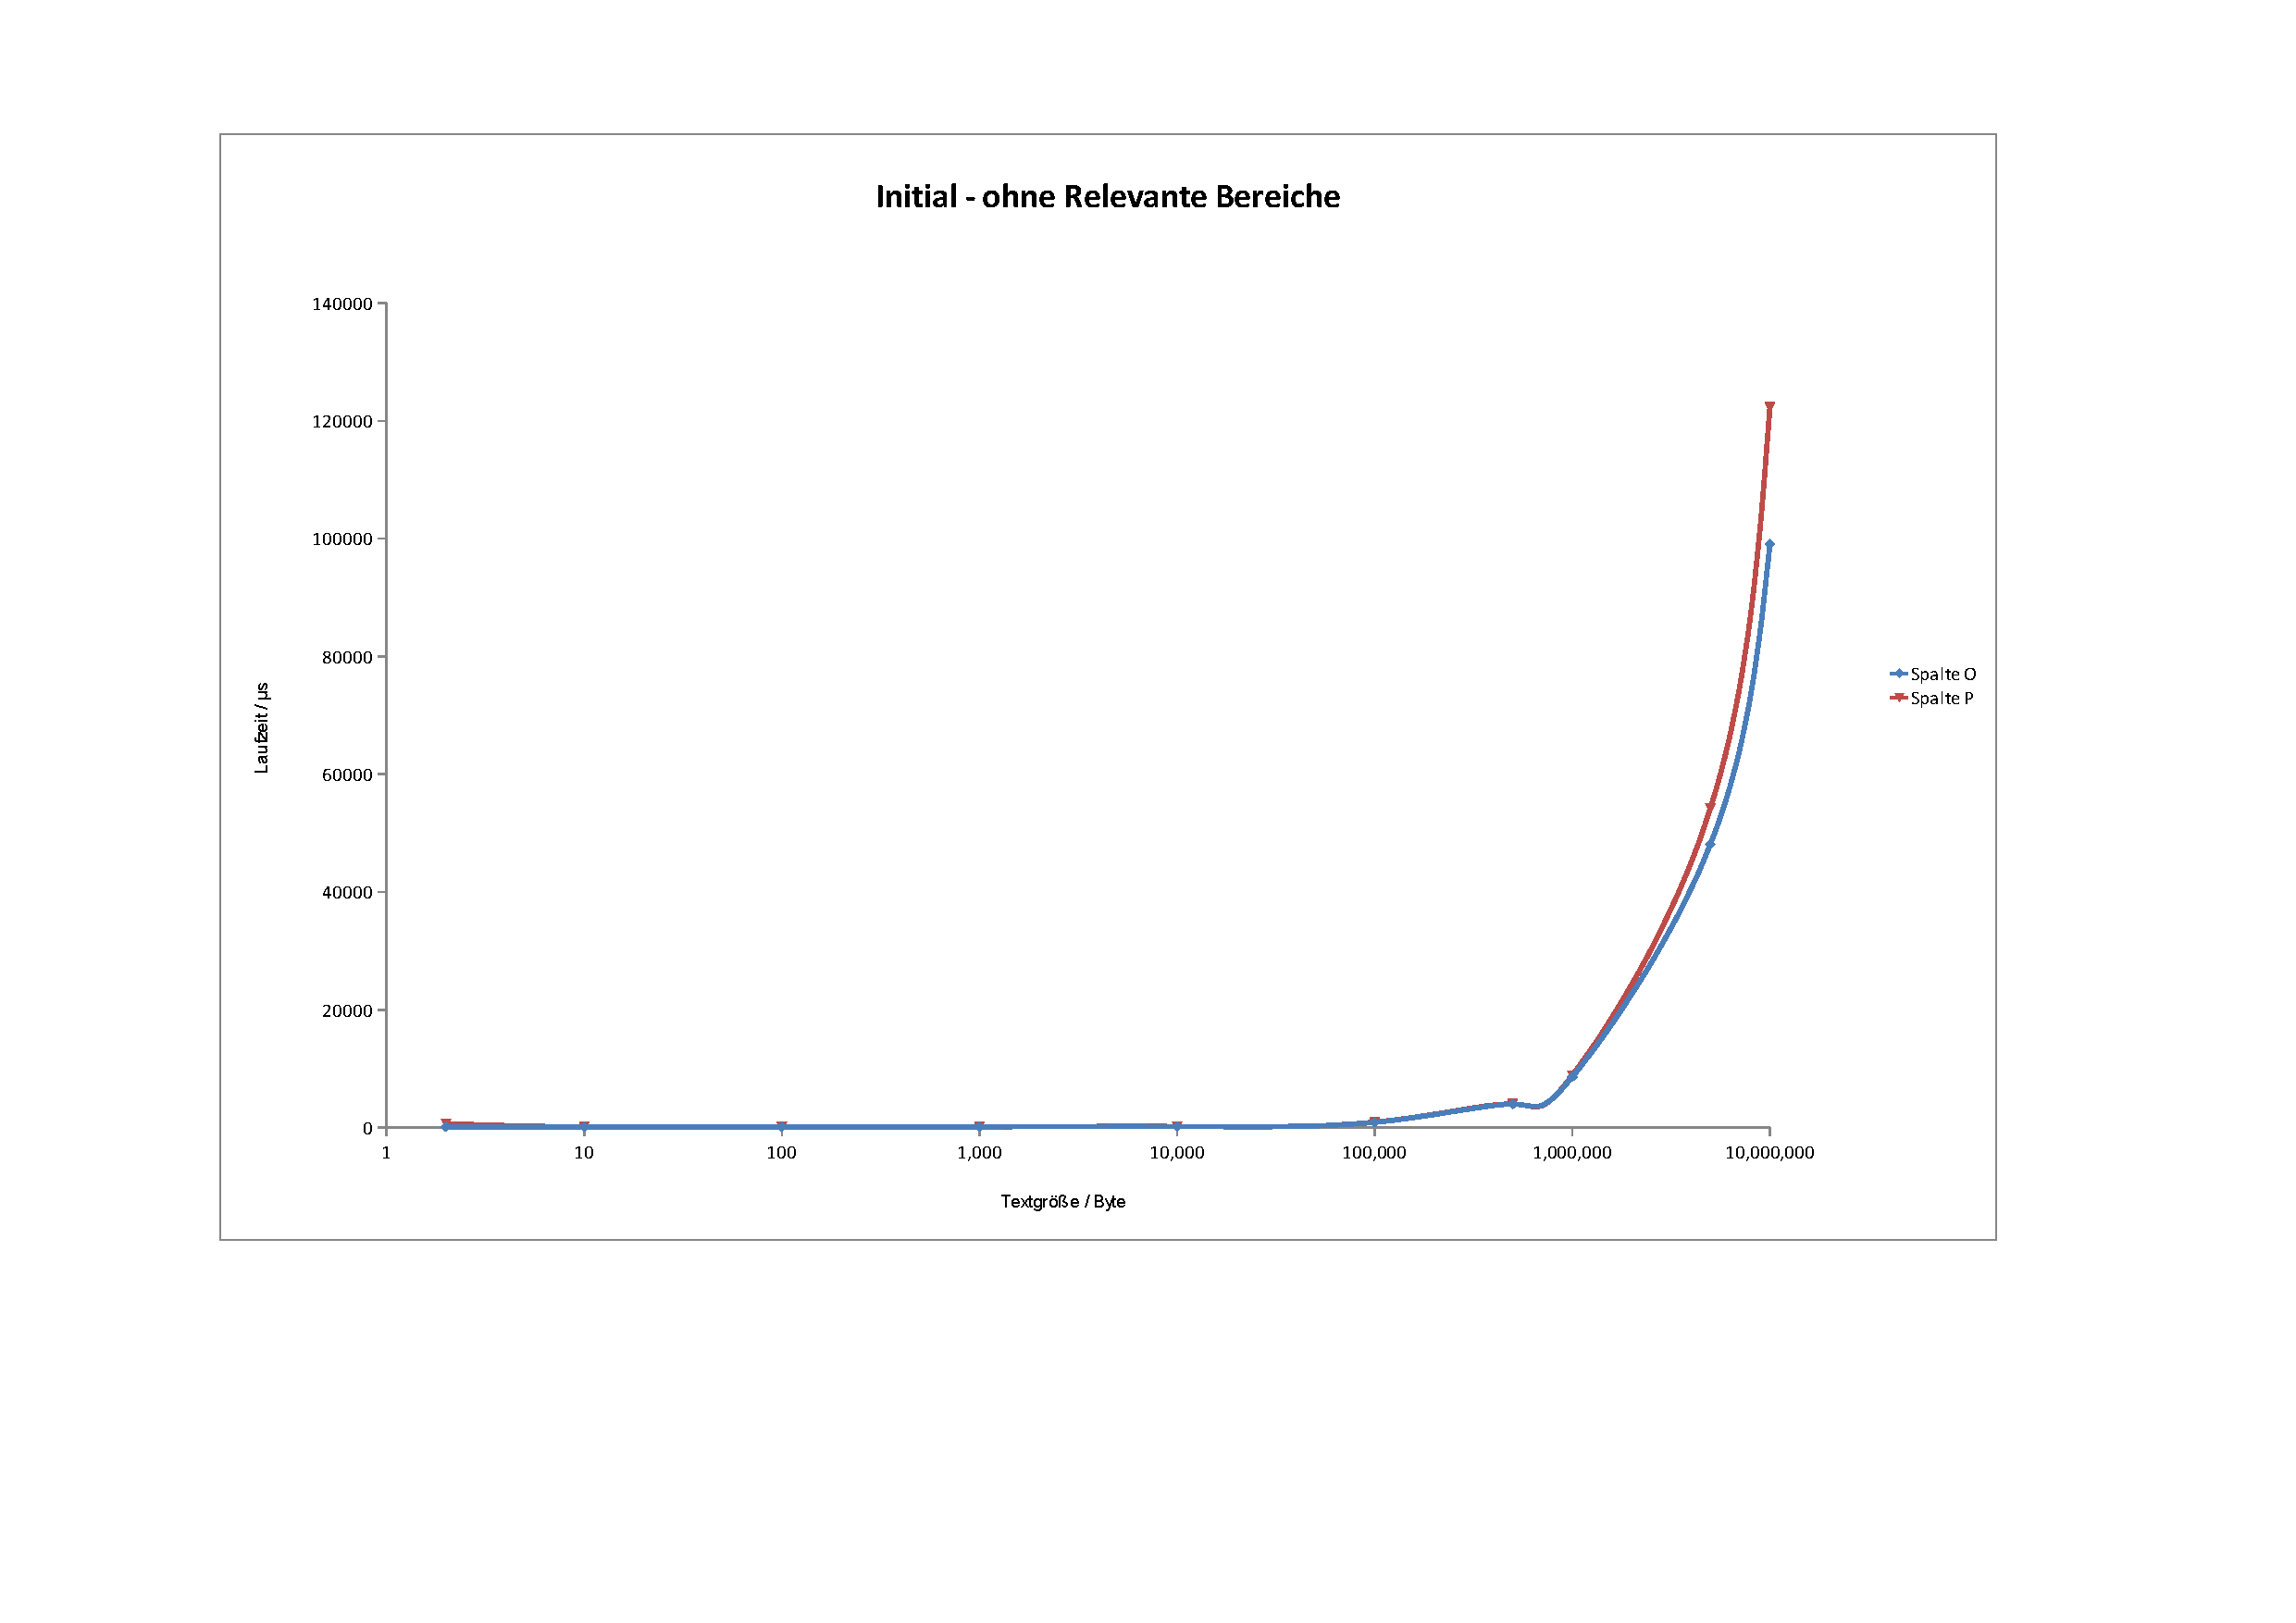
\includegraphics[scale=.45]{DiagrammInitial_worp.pdf}
	\label{fig:diagrammInitial_wrp}
	\caption{Messung-Initial ohne relevante Bereiche}
\end{figure}

In Abbildung \ref{fig:diagrammInitial_wrp} ist die Laufzeit bezüglich
verschiedener Anzahlen relevanter Bereiche dargestellt. Die Textgröße bleibt
dabei stetig bei $5.000.000$ Byte. Damit ist ein Vergleich der Werte mit den
durchschnittlichen Werten der gleichen Textgröße aus Abbildung
\ref{fig:diagrammInitial_worp} möglich. Für nur wenige relevante Bereiche
unterscheiden sich die Werte maginal. Steigt die Anzahl, nimmt die Laufzeit
jedoch exponentiell zu (siehe Abbildung \ref{fig:diagrammInitial}) und bewegen
sich im Millisekunden-Bereich. Dies Bedeutet, dass die Implementierung noch
nicht für die Verwendung von einer sehr große Anzahl an relevanten Bereichen
optimiert wurde. Im Kapitel \ref{sec:Anwendungsszenarien} wurden bereits
mögliche Anwendungsszenarien betrachtet, welche ebenso mit wenigen relevanten
Bereichen auskommen. Dadurch ist eine Optimierung an dieser Stelle vorerst
nebensächlich.

\begin{figure}[H]
	\centering
	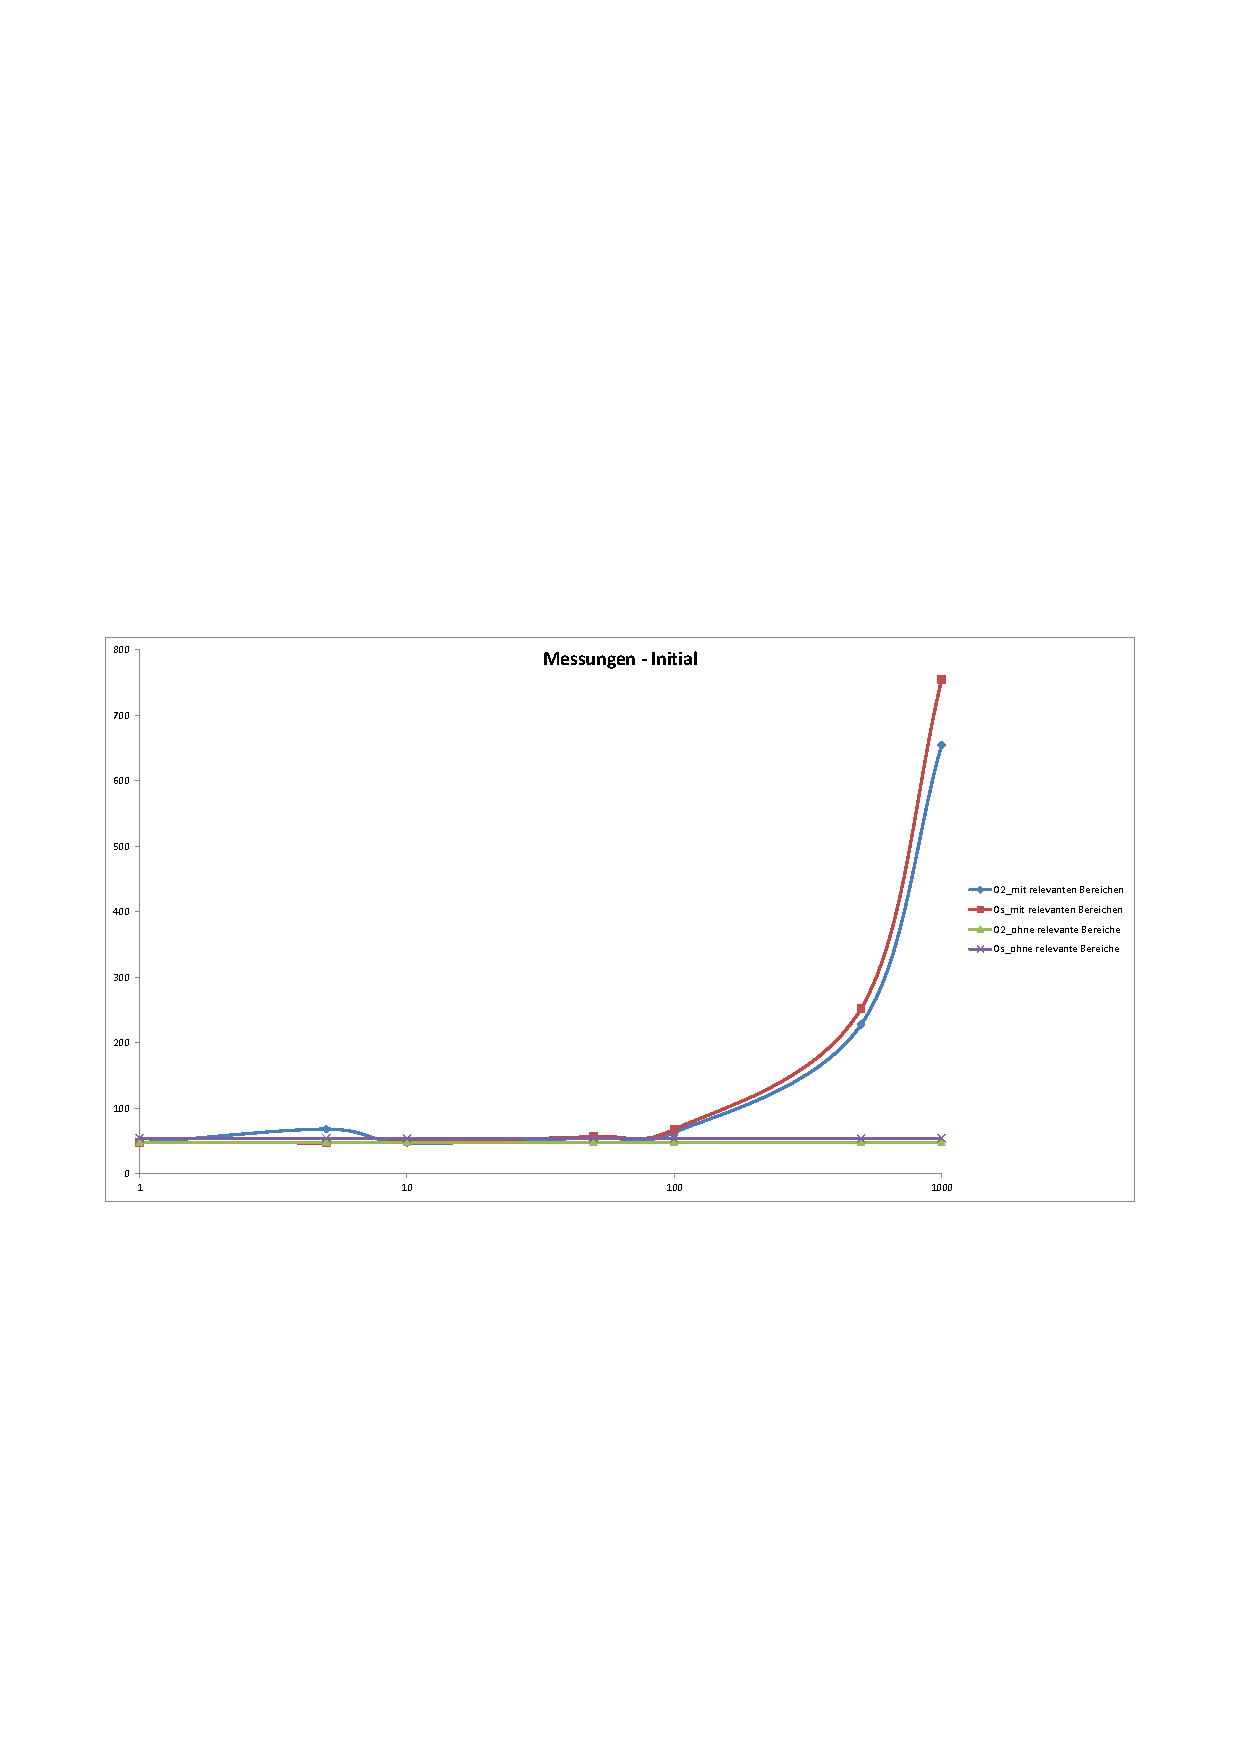
\includegraphics[width=\textwidth]{DiagrammInitial.pdf}
	\label{fig:diagrammInitial}
	\caption{Messung-Initial}
\end{figure}

Bei der letzten Messung werden nacheinander unterschiedliche
Datengrößen und zusätzlich Daten mit unterschiedlicher Anzahl an relevanten
Bereichen betrachtet. Dabei wird das Modul nicht neu erstellt. Hierbei ist zu
erkennen, dass die Verarbeitungsdauer ansteigt, je mehr Daten schon bearbeitet
wurden. Eine genauere Analyse zeigt, dass die priorisierenden \gls{FIFO} der
Flaschenhals ist. Bei diesem Testdurchlauf wurden insgesamt $41.400$ Datenblöcke
aus $548$ MB verarbeitet.
Dabei lagen alle Datenblöcke gleichzeitig in der \gls{FIFO}, wodurch das Einsortieren neuer
Blöcke sehr viel Rechenleistung in Anspruch nimmt. Gleichzeitig werden diese
Daten im Arbeitsspeicher und auf der Festplatte gespeichert. Hierbei gilt zu
untersuchen, ob diese Form der Datensicherung bei einem Rover auf dem
Mars praktikabel ist, da dieser über sehr begrenzte Speicherressourcen verfügt.
Alternativ müssen neue Methoden gefunden werden den Speicherverbrauch
einzuschränken. So besteht die Möglichkeit die Daten nur auf der Festplatte
zu speichern und in der \gls{FIFO} die Indizies zu diesen zu hinterlegen,
wodurch der Speicherverbrauch im Arbeitsspeicher stark reduziert werden kann.
Allerdings ist diese Methode bei sehr vielen Daten nicht optimal, welche sich
bei sehr langen Zeiträumen in denen nicht gesendet werden kann ansammeln.
Eine bessere Möglichkeit wäre anhand einer \gls{TTL} (siehe Kapitel
\ref{sec:Vorueberlegung}) unrelevante Daten nur sehr kurzfristig vorzuhalten, damit mehr Raum für Daten
von hoher Relevanz ist.
